\documentclass{article}
\usepackage[margin=1in]{geometry}
\usepackage{graphicx}
\usepackage{xcolor}
\usepackage{float}
\usepackage{amsmath}
\usepackage{cite}
\usepackage{hyperref}
\usepackage{indentfirst}
\graphicspath{{..} {./images}}

\definecolor{navy-blue}{rgb}{0.22,0.38,0.71}

\renewcommand{\contentsname}{\vspace*{-2\baselineskip}}

\hypersetup{
	colorlinks,
	linkcolor=black,
	urlcolor=blue,
	citecolor=black
}
  		
\begin{document}
\begin{titlepage}
	\centering
	{\huge Lab 4 - Analog Modulation with SDR}\\[0.25 in]
	
\includegraphics[width=0.6\textwidth]{ua_logo.png}\\[0.25 in]
	{\large \textbf{ECE 531 - Software Defined Radio\\[0.25 in]
	March 17, 2025\\[0.25 in]}}
	{\large Owen Sowatzke, osowatzke@arizona.edu\\[0.05 in]
	Department of Electrical \& Computer Engineering\\[0.05 in]
	University of Arizona, Tucson, AZ 85721\\[0.5 in]}
	\hypersetup{linkcolor=navy-blue}
	\noindent\hrulefill
	\tableofcontents
	\noindent\hrulefill
\end{titlepage}

% \setlength{\parindent}{0pt}

\section{Introduction}
%Introduction to the laboratory experiment, including a brief description of the objectives and goals.

\section{Procedure}
% Detailed explanation of the laboratory experiment, including the design, implementation, and testing of the system.

\subsection{FM Demodulation using GNU Radio}
\label{section::fm_demod_gnu_radio}

In this experiment, we use the GNU radio flowchart shown in Figure \ref{fig::fm_radio_flowchart} to perform FM demodulation.

\begin{figure}[H]
	\centerline{\fbox{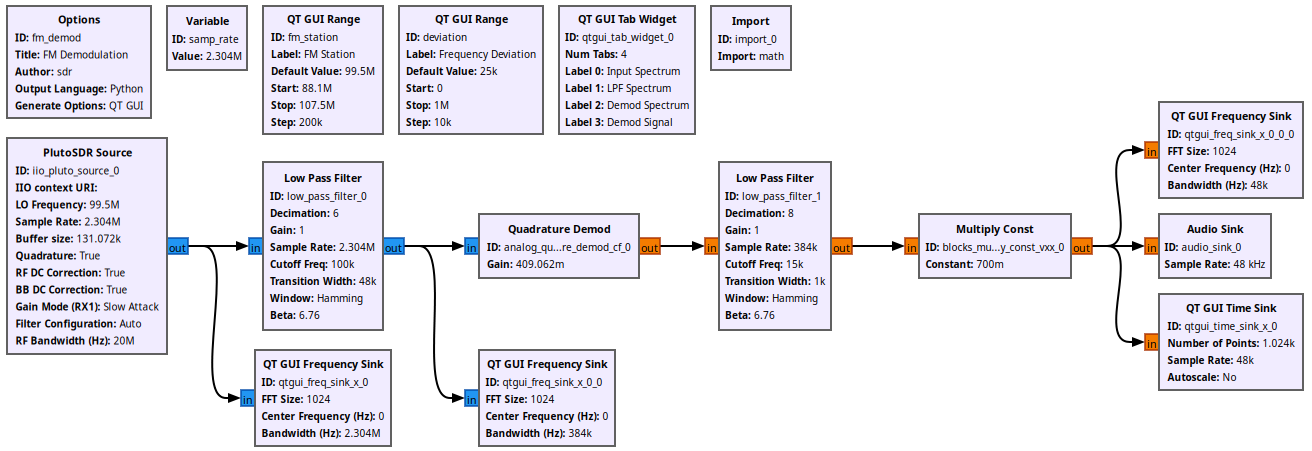
\includegraphics[width=0.7\textwidth]{fm_radio_flowchart.png}}}
	\caption{Flowchart for FM Demodulation}
	\label{fig::fm_radio_flowchart}
\end{figure}

\noindent Using the flowchart, we capture images of the spectrum before and and after demodulation. We also turn on averaging to reduce the variance of the noise floor. This allows us to better visualize the FM spectrum. Next, we list the decimation blocks in the flowchart and explain why they are needed. Then, we discuss when a rational resampler block is needed and why it is not needed for the flowchart shown in Figure \ref{fig::fm_radio_flowchart}. Using the flowchart, we analyze the quality of the audio output and describe what modifications can be made to improve the audio quality. Finally, we justify the 100 kHz cutoff frequency of the low-pass filter (LPF).

\subsection{Manual RF Demodulation}

In this experiment, we repeat the analysis from Section \ref{section::fm_demod_gnu_radio} using a quadrature demodulator and low-pass filter instead of a FM demodulator block. Using the flowchart, we specifically capture images of the spectrum before and after demodulation. We also enable spectral averaging as we did above. Then, we examine the role of decimation, interpolation, and resampling blocks in our flowchart. We also compare the audio quality to the audio quality in the above flowchart and describe how we might improve the audio output.

\section{Results}
% Results and discussion of the laboratory experiment, including captured outputs, observations, and responses to laboratory questions.

\subsection{FM Demodulation using GNU Radio}

In this section, we use the flowchart shown in Figure \ref{fig::fm_radio_flowchart} to receive, demodulate, and play audio from FM radio signals. We specifically tune the flowchart to 99.5 MHz (99.5 FM) and capture the spectrum before and after demodulation. The input spectrum is captured in Figure \ref{fig::fm_radio_input_spectrum}.

\begin{figure}[H]
	\centerline{\fbox{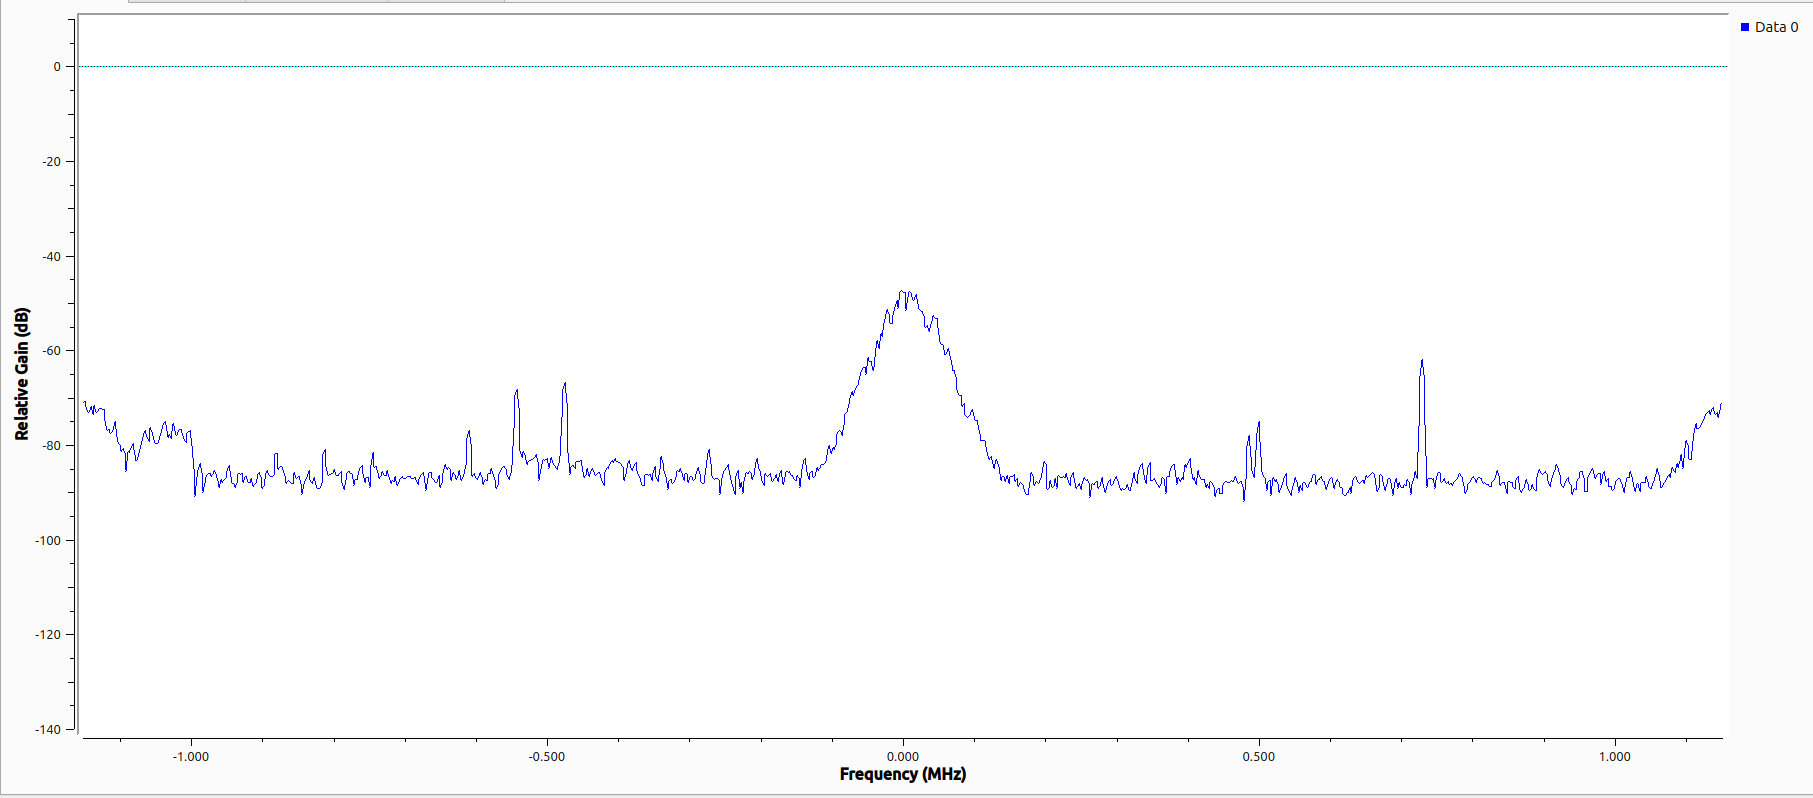
\includegraphics[width=0.7\textwidth]{fm_radio_input_spectrum.png}}}
	\caption{FM Radio Input Spectrum}
	\label{fig::fm_radio_input_spectrum}
\end{figure}

\noindent Looking at the input spectrum, we see that FM radio signal is centered at the middle of the band. We also see that the signal is sampled at a rate much higher than the input bandwidth. Next, we analyze the spectrum after the LPF and a decimation of 6. The resulting spectrum is shown in Figure \ref{fig::fm_radio_lpf_spectrum}.

\begin{figure}[H]
	\centerline{\fbox{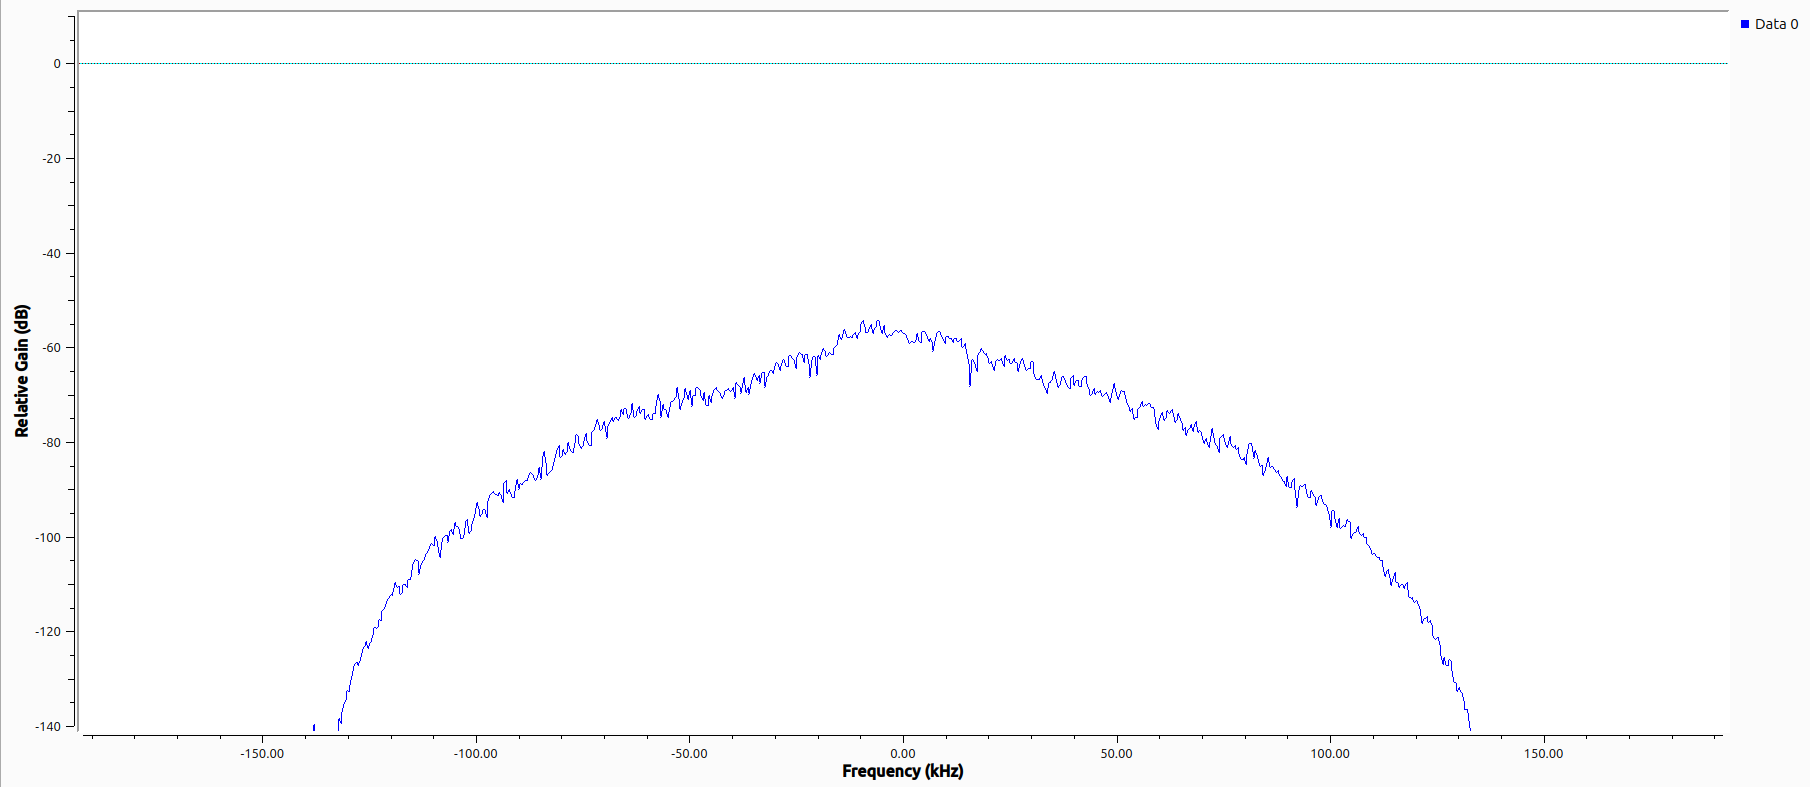
\includegraphics[width=0.7\textwidth]{fm_radio_lpf_spectrum.png}}}
	\caption{FM Radio LPF Spectrum}
	\label{fig::fm_radio_lpf_spectrum}
\end{figure}

\noindent Examining the low pass filter output, we see that we have passed most of the FM radio spectrum. We also see that we have properly band-limited our signal to prevent aliasing during decimation. Finally, we examine the spectrum of the demodulated signal, which is shown in Figure \ref{fig::fm_radio_demod_spectrum}.

\begin{figure}[H]
	\centerline{\fbox{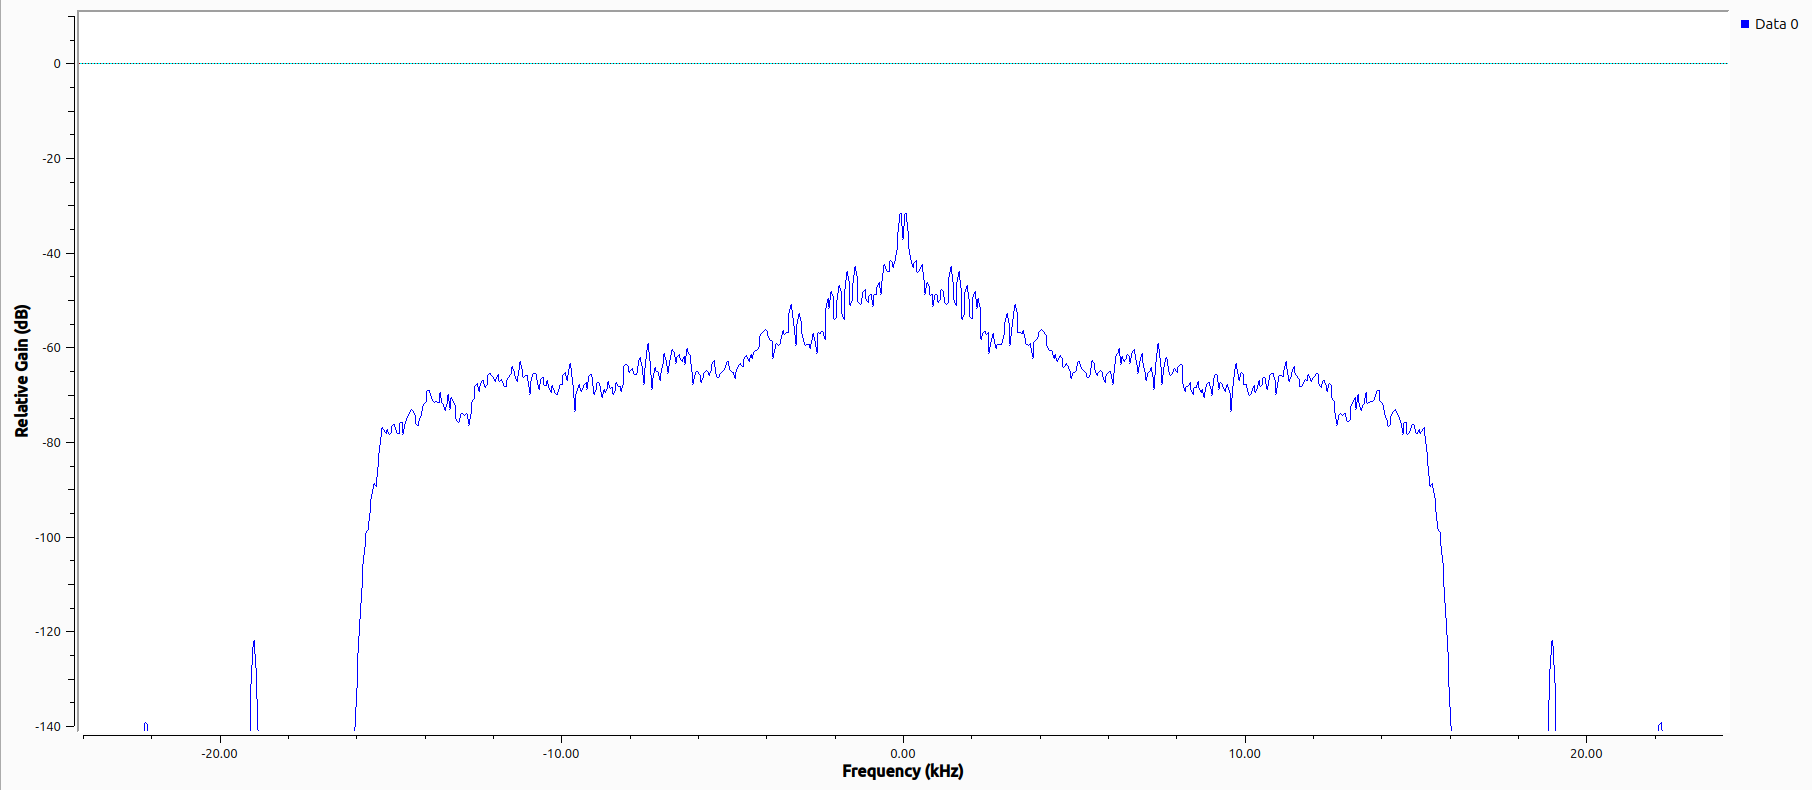
\includegraphics[width=0.7\textwidth]{fm_radio_demod_spectrum.png}}}
	\caption{Demodulated FM Signal Spectrum}
	\label{fig::fm_radio_demod_spectrum}
\end{figure}

\noindent Note that the spectrum of the demodulated signal is very different than the input spectrum. This is because the demodulation block returns a filtered copy of the signal phase. Note that the filter cutoff frequency is approximately 15 kHz, which is sufficient for audio signals. The filtering also prevents aliasing when we decimate the signal to the 48 kHZ audio output rate.

As hinted at above, there are two decimating filters within the block diagram. One is before the FM demodulation block and limits the bandwidth of the signal to the width of the RF channel. The second filter is included with the FM demodulation block, and it limits the frequency of the audio output for the audio sink. The first filter includes a decimate by 6, and the second filter includes a decimate by 8. As a result, our sample rate falls from 2.304 MHz to 48 kHz. Note that this decimation is important because we must feed the audio source at a rate of 48 kHz.

In the flowchart, a rational resampler block is needed instead of decimating FIRs if the input sampling rate is not a multiple of the audio sink sampling rate. In Figure \ref{fig::fm_radio_flowchart}, the input sampling rate is a multiple of the audio sink sampling rate (i.e. $48\ \text{kHz} \times 48 = 2.304\ \text{MHz}$). Therefore, a rational resampler block is not needed.

The FM radio sound quality from our flowchart is pretty good. However, we can improve the SNR of our signal, by decreasing the RF bandwidth. Our initial RF bandwidth of 20 MHz is larger than the sampling rate of 2.304 MHz, which allows some spectral content to alias. FM radio channels have a bandwidth of 200 kHz, so we want a sample rate larger than 200 kHz and less than the sampling rate of 2.304 MHz. The RF filter is not perfect, so we should choose a bandwidth in the middle of this range to minimize the attenuation of our signal bandwidth and out-of-band aliasing. The 100 MHz cutoff frequency for the low-pass filter (LPF) is sized to the 200 MHZ bandwidth of the FM radio signal instead of the LPF sampling rate. Because the filter bandwidth is less than the sampling rate, we will not have problems with aliasing. Additionally, the reduced bandwidth fully captures our signal, while reducing the amount of noise entering the FM demodulator.

\subsection{Manual RF Demodulation}

\begin{figure}[H]
	\centerline{\fbox{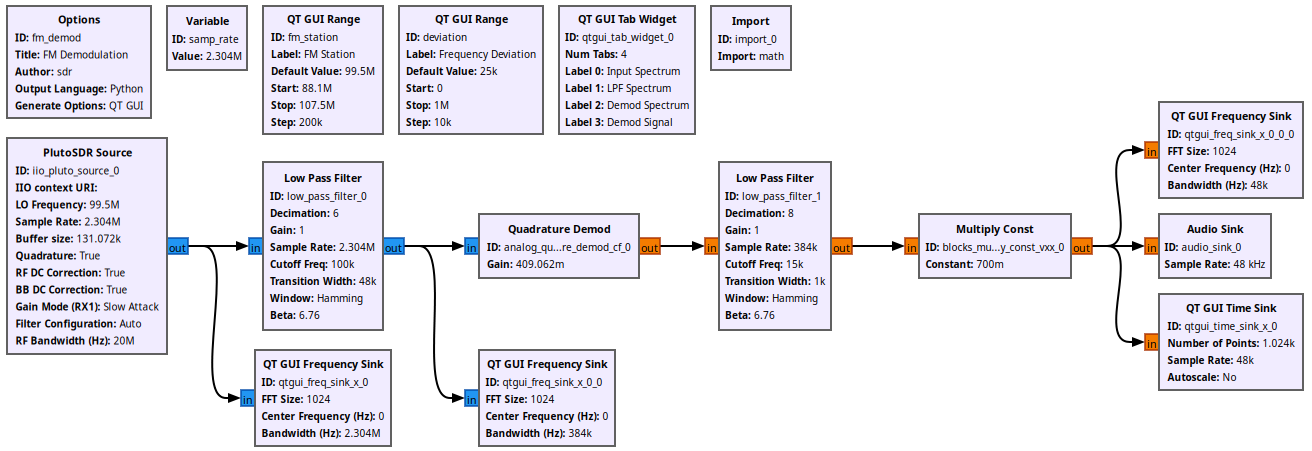
\includegraphics[width=0.7\textwidth]{fm_radio_user_flowchart.png}}}
	\caption{FM Radio Flowchart with Custom Blocks}
	\label{fig::fm_radio_user_flowchart}
\end{figure}

\begin{figure}[H]
	\centerline{\fbox{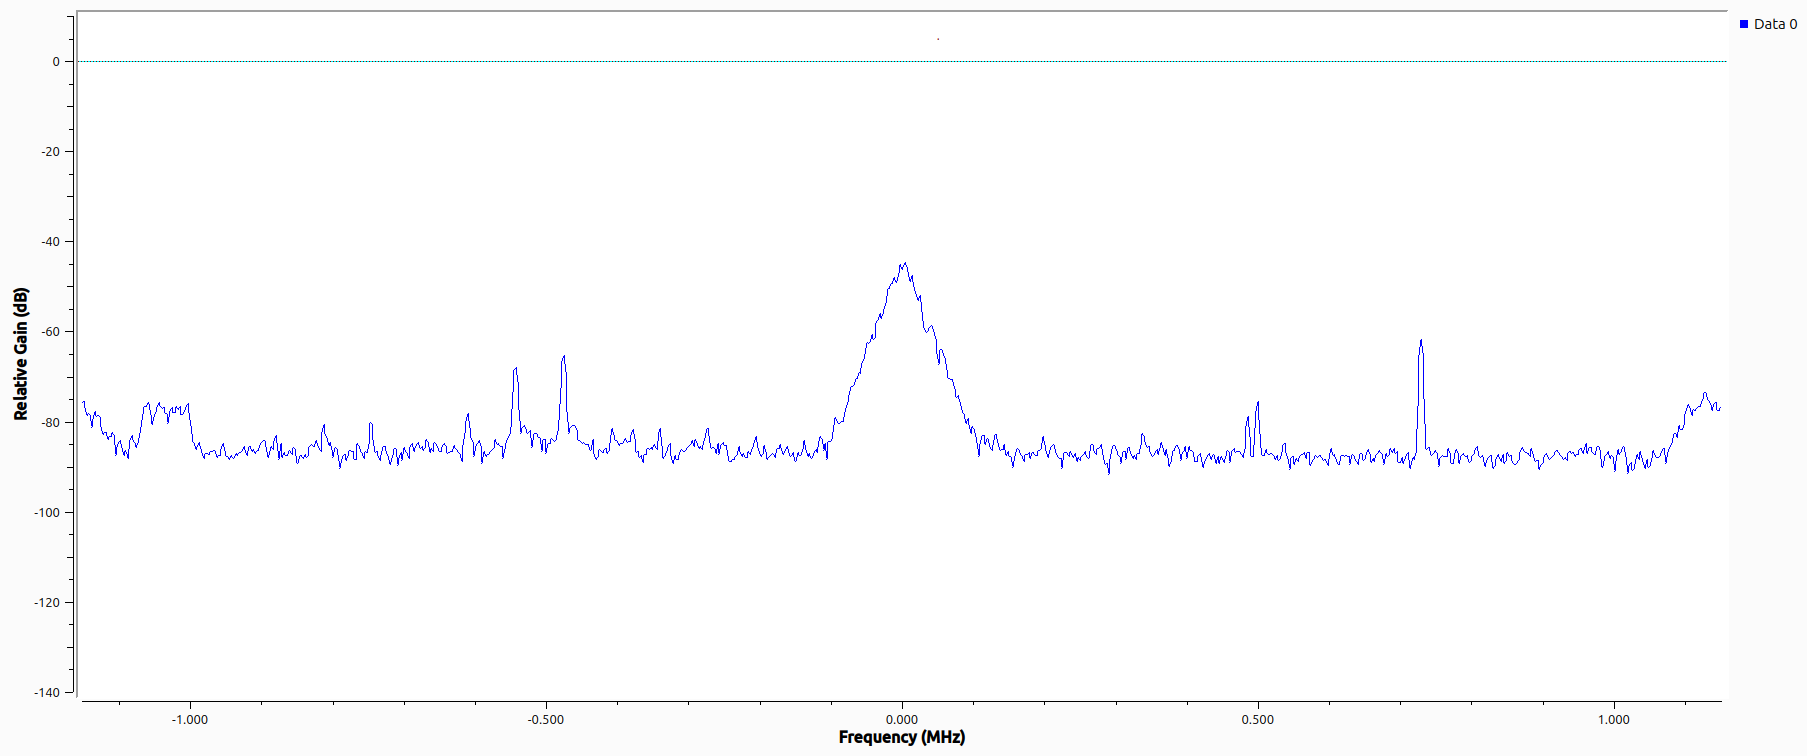
\includegraphics[width=0.7\textwidth]{fm_radio_user_input_spectrum.png}}}
	\caption{FM Radio Input Spectrum}
	\label{fig::fm_radio_user_input_spectrum}
\end{figure}

\begin{figure}[H]
	\centerline{\fbox{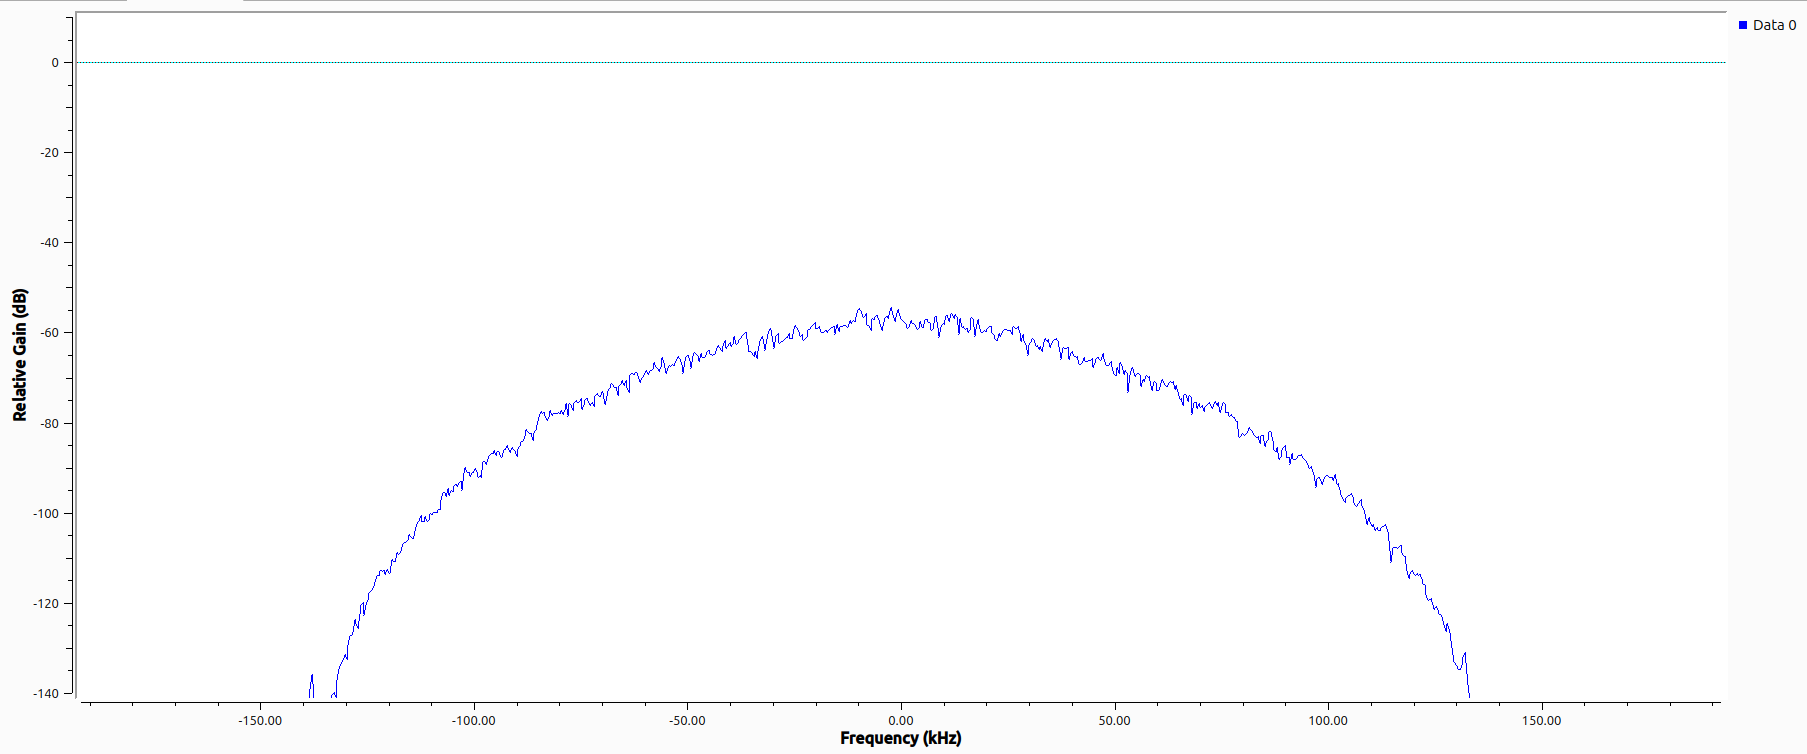
\includegraphics[width=0.7\textwidth]{fm_radio_user_lpf_spectrum.png}}}
	\caption{FM Radio LPF Spectrum}
	\label{fig::fm_radio_user_lpf_spectrum}
\end{figure}

\begin{figure}[H]
	\centerline{\fbox{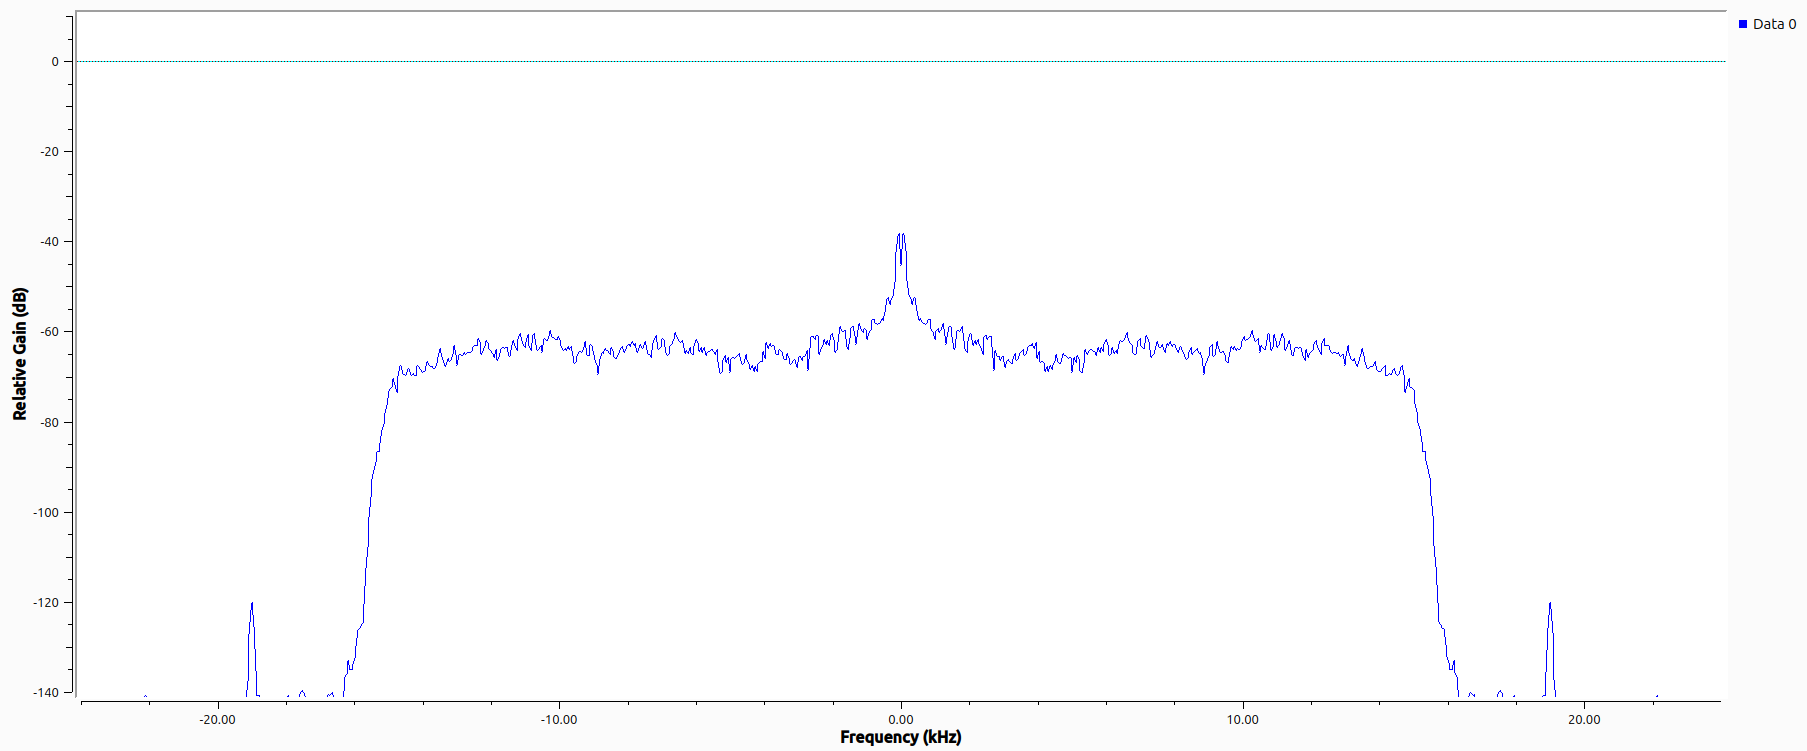
\includegraphics[width=0.7\textwidth]{fm_radio_user_demod_spectrum.png}}}
	\caption{Demodulated FM Signal Spectrum}
	\label{fig::fm_radio_user_demod_spectrum}
\end{figure}

\subsection{Questions}

In this section, we answer questions about AM modulation. Note that we cannot demodulate AM radio in the PlutoSDR, without additional hardware such as an upconverter. This is because the AM radio band (530 kHz - 1700 kHz) is outside of the Pluto's operating frequencies (70 MHz - 6 GHz). Car stereos, on the other hand, are specifically designed to receive signals in this band and do not require additional hardware.

Due to these deficiencies, we simply discuss the demodulation that we would perform if we had the additional hardware. The "AM Demod" block in GNU radio, is typically used to perform this demodulation. However, we can instead use a "Complex to Mag" block followed by a bandpass filter. Note that we use a bandpass filter instead of a low-pass filter to remove the carrier signal that is transmitted with the AM signal.
  
\section{Conclusion}
% Conclusions to the overall lab that discuss meaningful lessons learned and other takeaways from the assignment. (Important)

%\nocite{analog_devices_libiio_error}
%\bibliographystyle{IEEEtran}
%\bibliography{sources}{}
%\bibliographystyle{ieeetr}
	
\end{document}